\rule{0.5\textwidth}{0.5pt}\\

	{\large \textbf{EXPERIMENT Euclidean distances}}\\
	
	\begin{figure*}[ht!]
		\centering
		\subfloat[Train subset 0]{%
		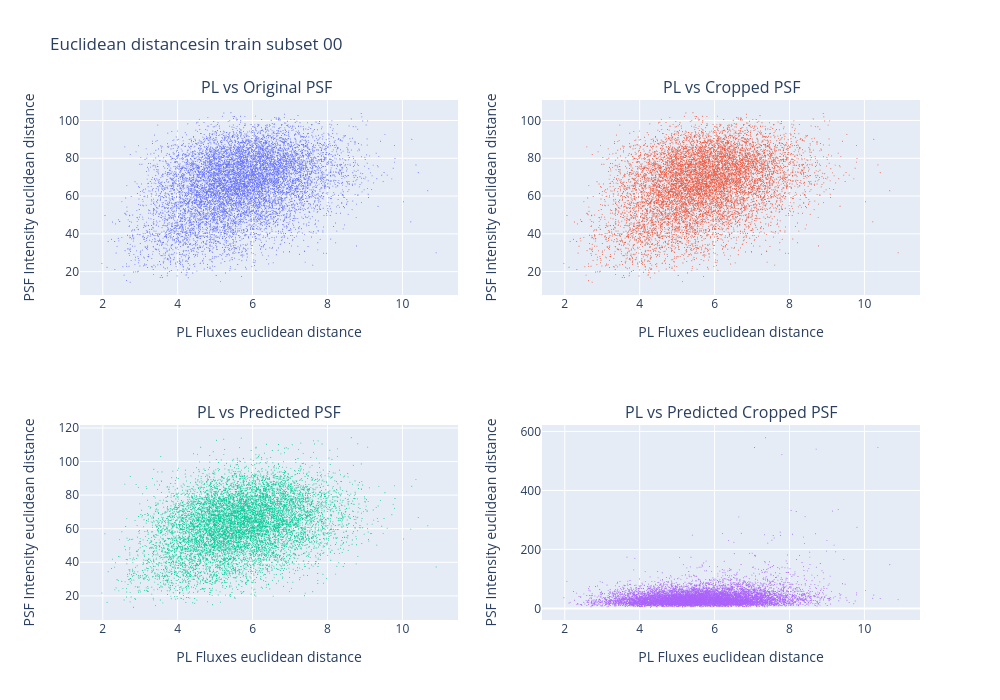
\includegraphics[width=0.45\textwidth]{euclideans_00.png}}
		\subfloat[Train subset 1]{%
		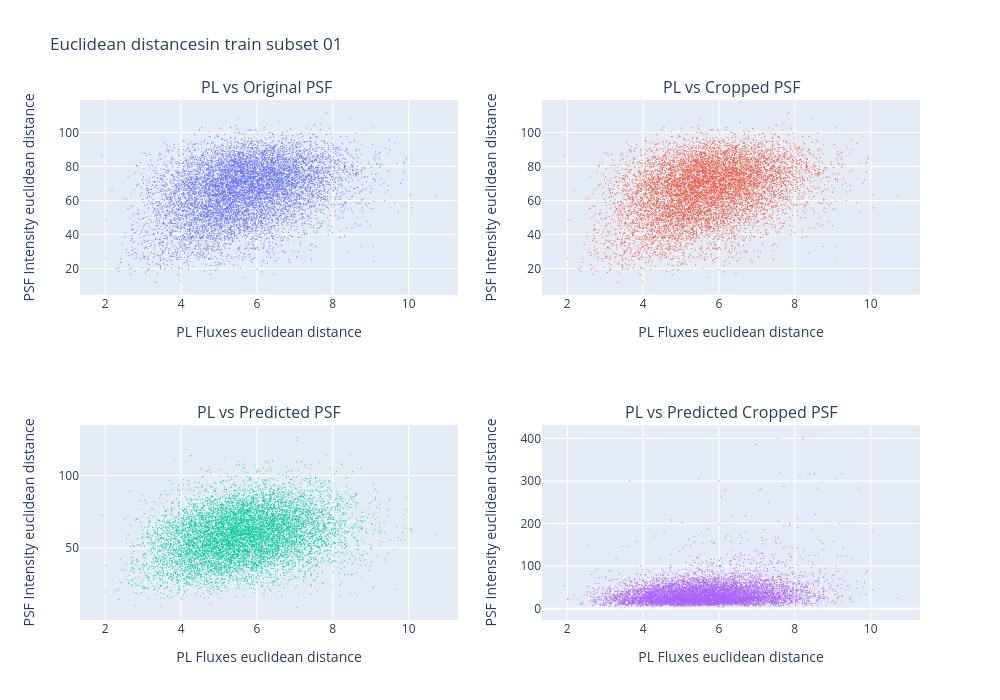
\includegraphics[width=0.45\textwidth]{euclideans_01.png}}\\
		\subfloat[Train subset 2]{%
		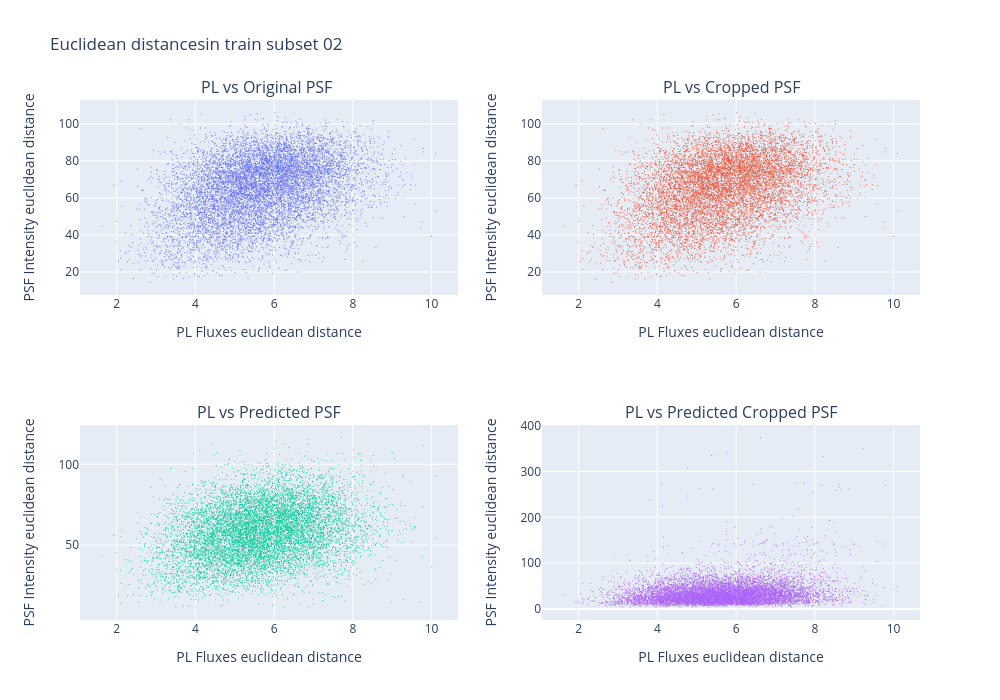
\includegraphics[width=0.45\textwidth]{euclideans_02.png}}
		\subfloat[Train subset 3]{%
		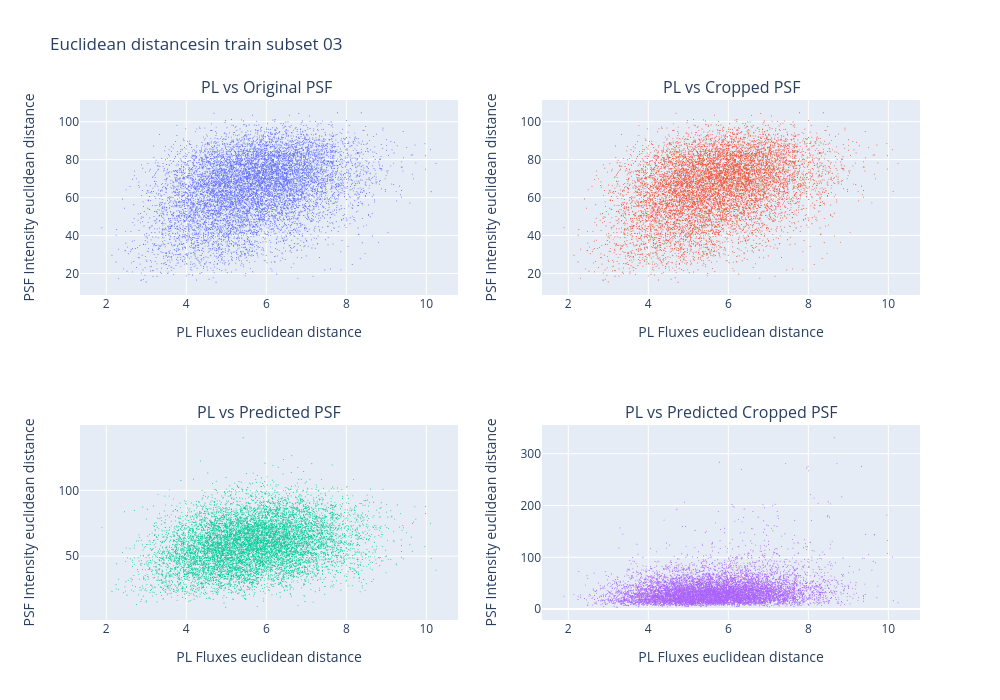
\includegraphics[width=0.45\textwidth]{euclideans_03.png}}\\
		\subfloat[Train subset 4]{%
		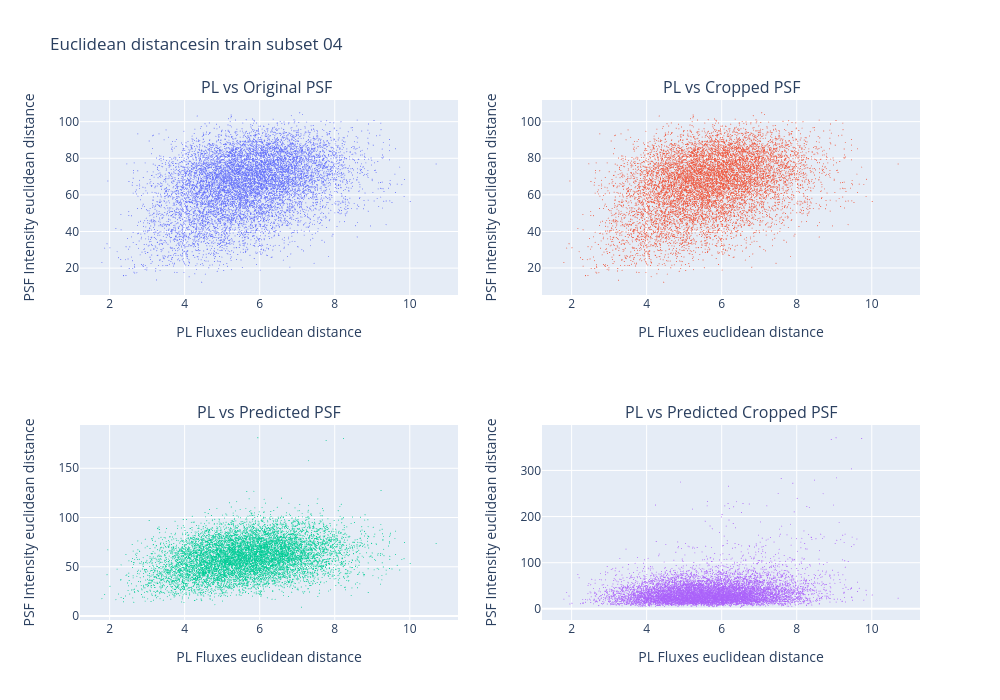
\includegraphics[width=0.45\textwidth]{euclideans_04.png}}
		\subfloat[Train subset 5]{%
		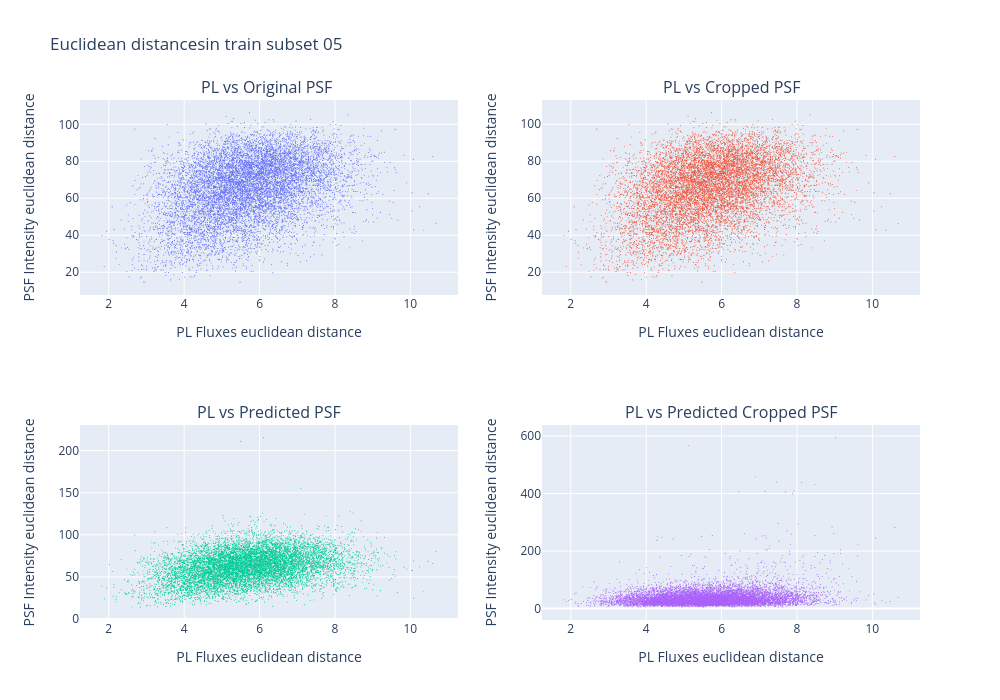
\includegraphics[width=0.45\textwidth]{euclideans_05.png}}\\
		\subfloat[Train subset 6]{%
		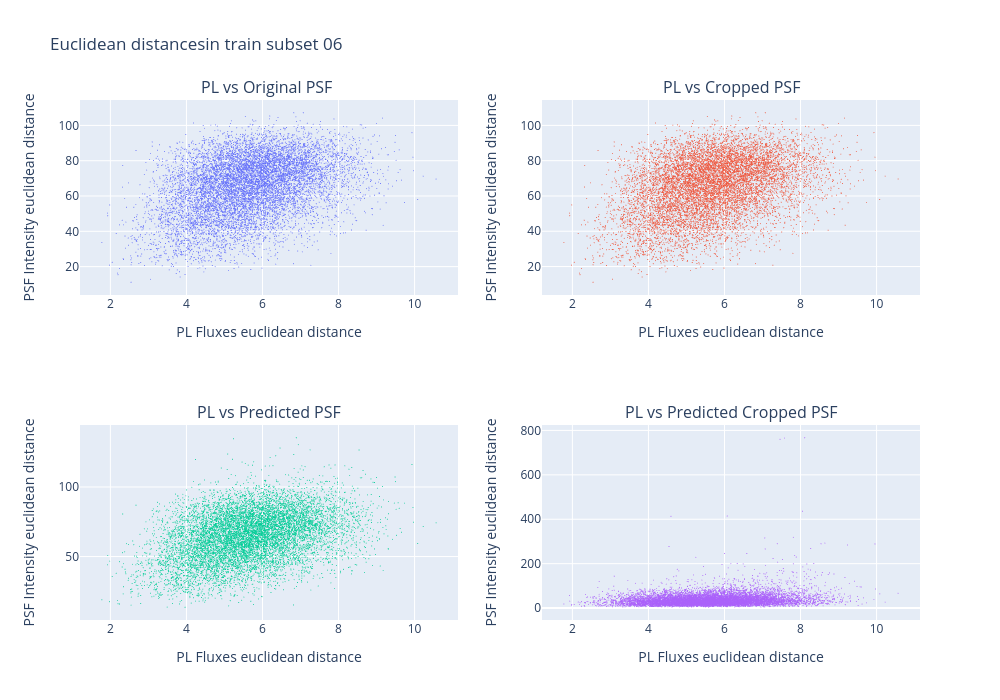
\includegraphics[width=0.45\textwidth]{euclideans_06.png}}
		\caption{Euclidean distances between PL and PSF pairs}\hspace{\fill}
	\end{figure*}
	
\FloatBarrier	
\rule{0.5\textwidth}{0.5pt}\\